\documentclass[11pt]{article}
\usepackage[left=0.7in,right=0.7in,top=1in,bottom=0.7in]{geometry}
\usepackage{fancyhdr}
\usepackage{graphicx}
\graphicspath{ {./images/} }
\usepackage[colorlinks=true]{hyperref}
\usepackage{lastpage}
\usepackage{float}

\newcommand{\manualVersion}{1.0}

\pagestyle{fancy}
\fancyhf{}
\fancyhead[L]{\textbf{SEED Labs - Open-Source CTF Platform Manual}}
\fancyhead[R]{Page {\thepage} of \pageref*{LastPage}}
\renewcommand{\headrulewidth}{1pt}

\begin{document}

\begin{center}
	{\Huge Open-Source CTF Platform Manual} \\
	{\small Version \manualVersion\ - \today}
\end{center}

\section{For Administrators}

\subsection{Videos}

The following videos show a quick walkthrough of setting up the SEED Labs CTF and a quick tour of its usage:

\begin{itemize}
	\item \href{run:./videos/SEED_CTF_setup_part1.mp4}{CTFd and \texttt{.zip} import}
	\item \href{run:./videos/SEED_CTF_setup_part2.mp4}{SEED Labs CTF tour}
\end{itemize}

\subsection{CTFd}

This project utilizes the open source \href{https://ctfd.io/}{CTFd} capture the flag platform to host the infrastructure needed to operate a successful capture the flag challenge.

\subsubsection{CTFd-as-a-service (hosted)}

CTFd offers a hosted version of the platform, in which they will set up the infrastructure needed to run CTFd and give you access to the management interface.
The CTFd hosted option is available for a cost, and more information can be found \href{https://ctfd.io/pricing/}{here}.

\subsubsection{Self-hosted}

Please follow the \href{https://docs.ctfd.io/docs/deployment/installation#docker}{CTFd Docker installation instructions} to install the platform on your own hardware.
By default CTFd does not have TLS enabled.
There are tutorials online for enabling TLS on your CTFd Docker instance.
For your convenience, \href{https://github.com/tghosth/CTFd-docker-deploy}{this is a third-party GitHub repo} with easy deployment instructions for CTFd with TLS enabled.
Once CTFd is installed and running you're able to import the provided CTF challenges into the platform.

\subsubsection{Admin Account Setup}

\begin{enumerate}
	\item Visit the CTFd site you launched above and click login.
   \begin{figure}[H]
		\centering
	   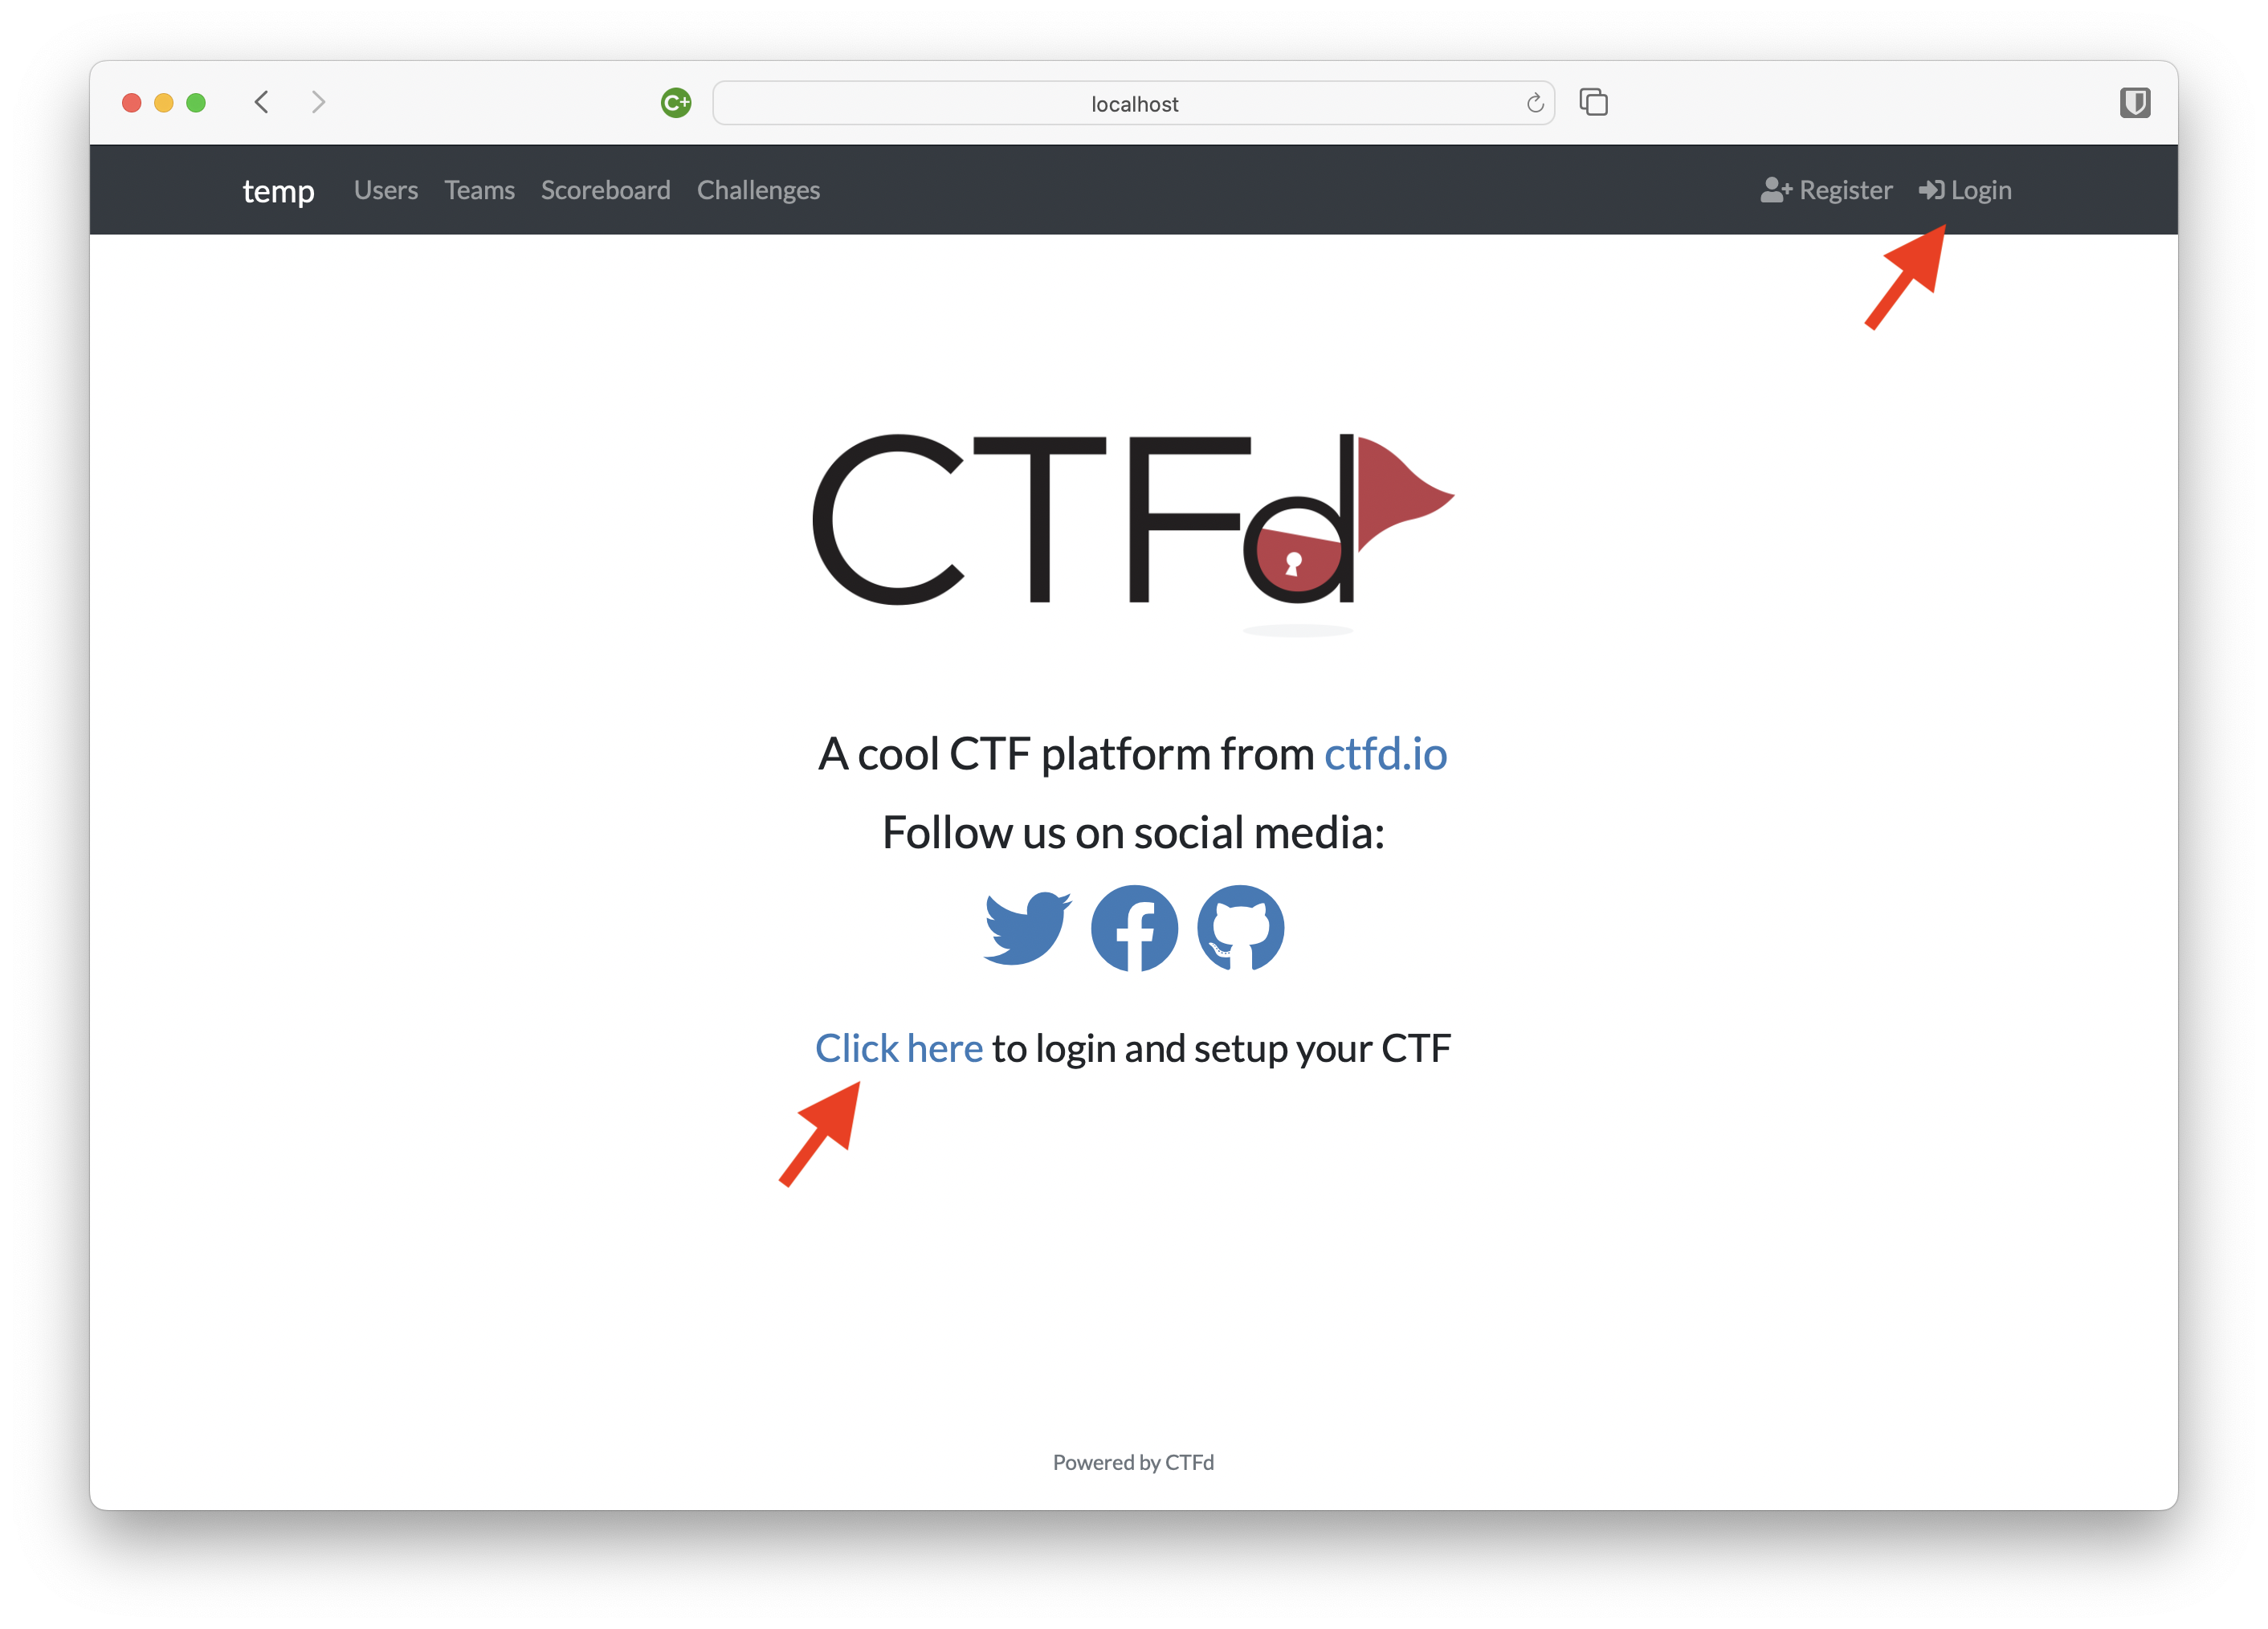
\includegraphics[width=\textwidth]{ctfd_landing_page.png}
  	   \caption{Click login on the CTFd landing page.}
	\end{figure}
	\item Login with default admin credentials (obtained by contacting the project maintainers; see bottom of page).
	\item Change the default admin credentials to your desired credentials (see below for procedure).
\end{enumerate}

\subsubsection{Changing Admin Account Credentials}

\begin{enumerate}
	
	\item Login with the default admin credentials (obtained by contacting the project maintainers; see bottom of page), then navigate to the admin panel.
	
	\begin{figure}[H]
		\centering
	   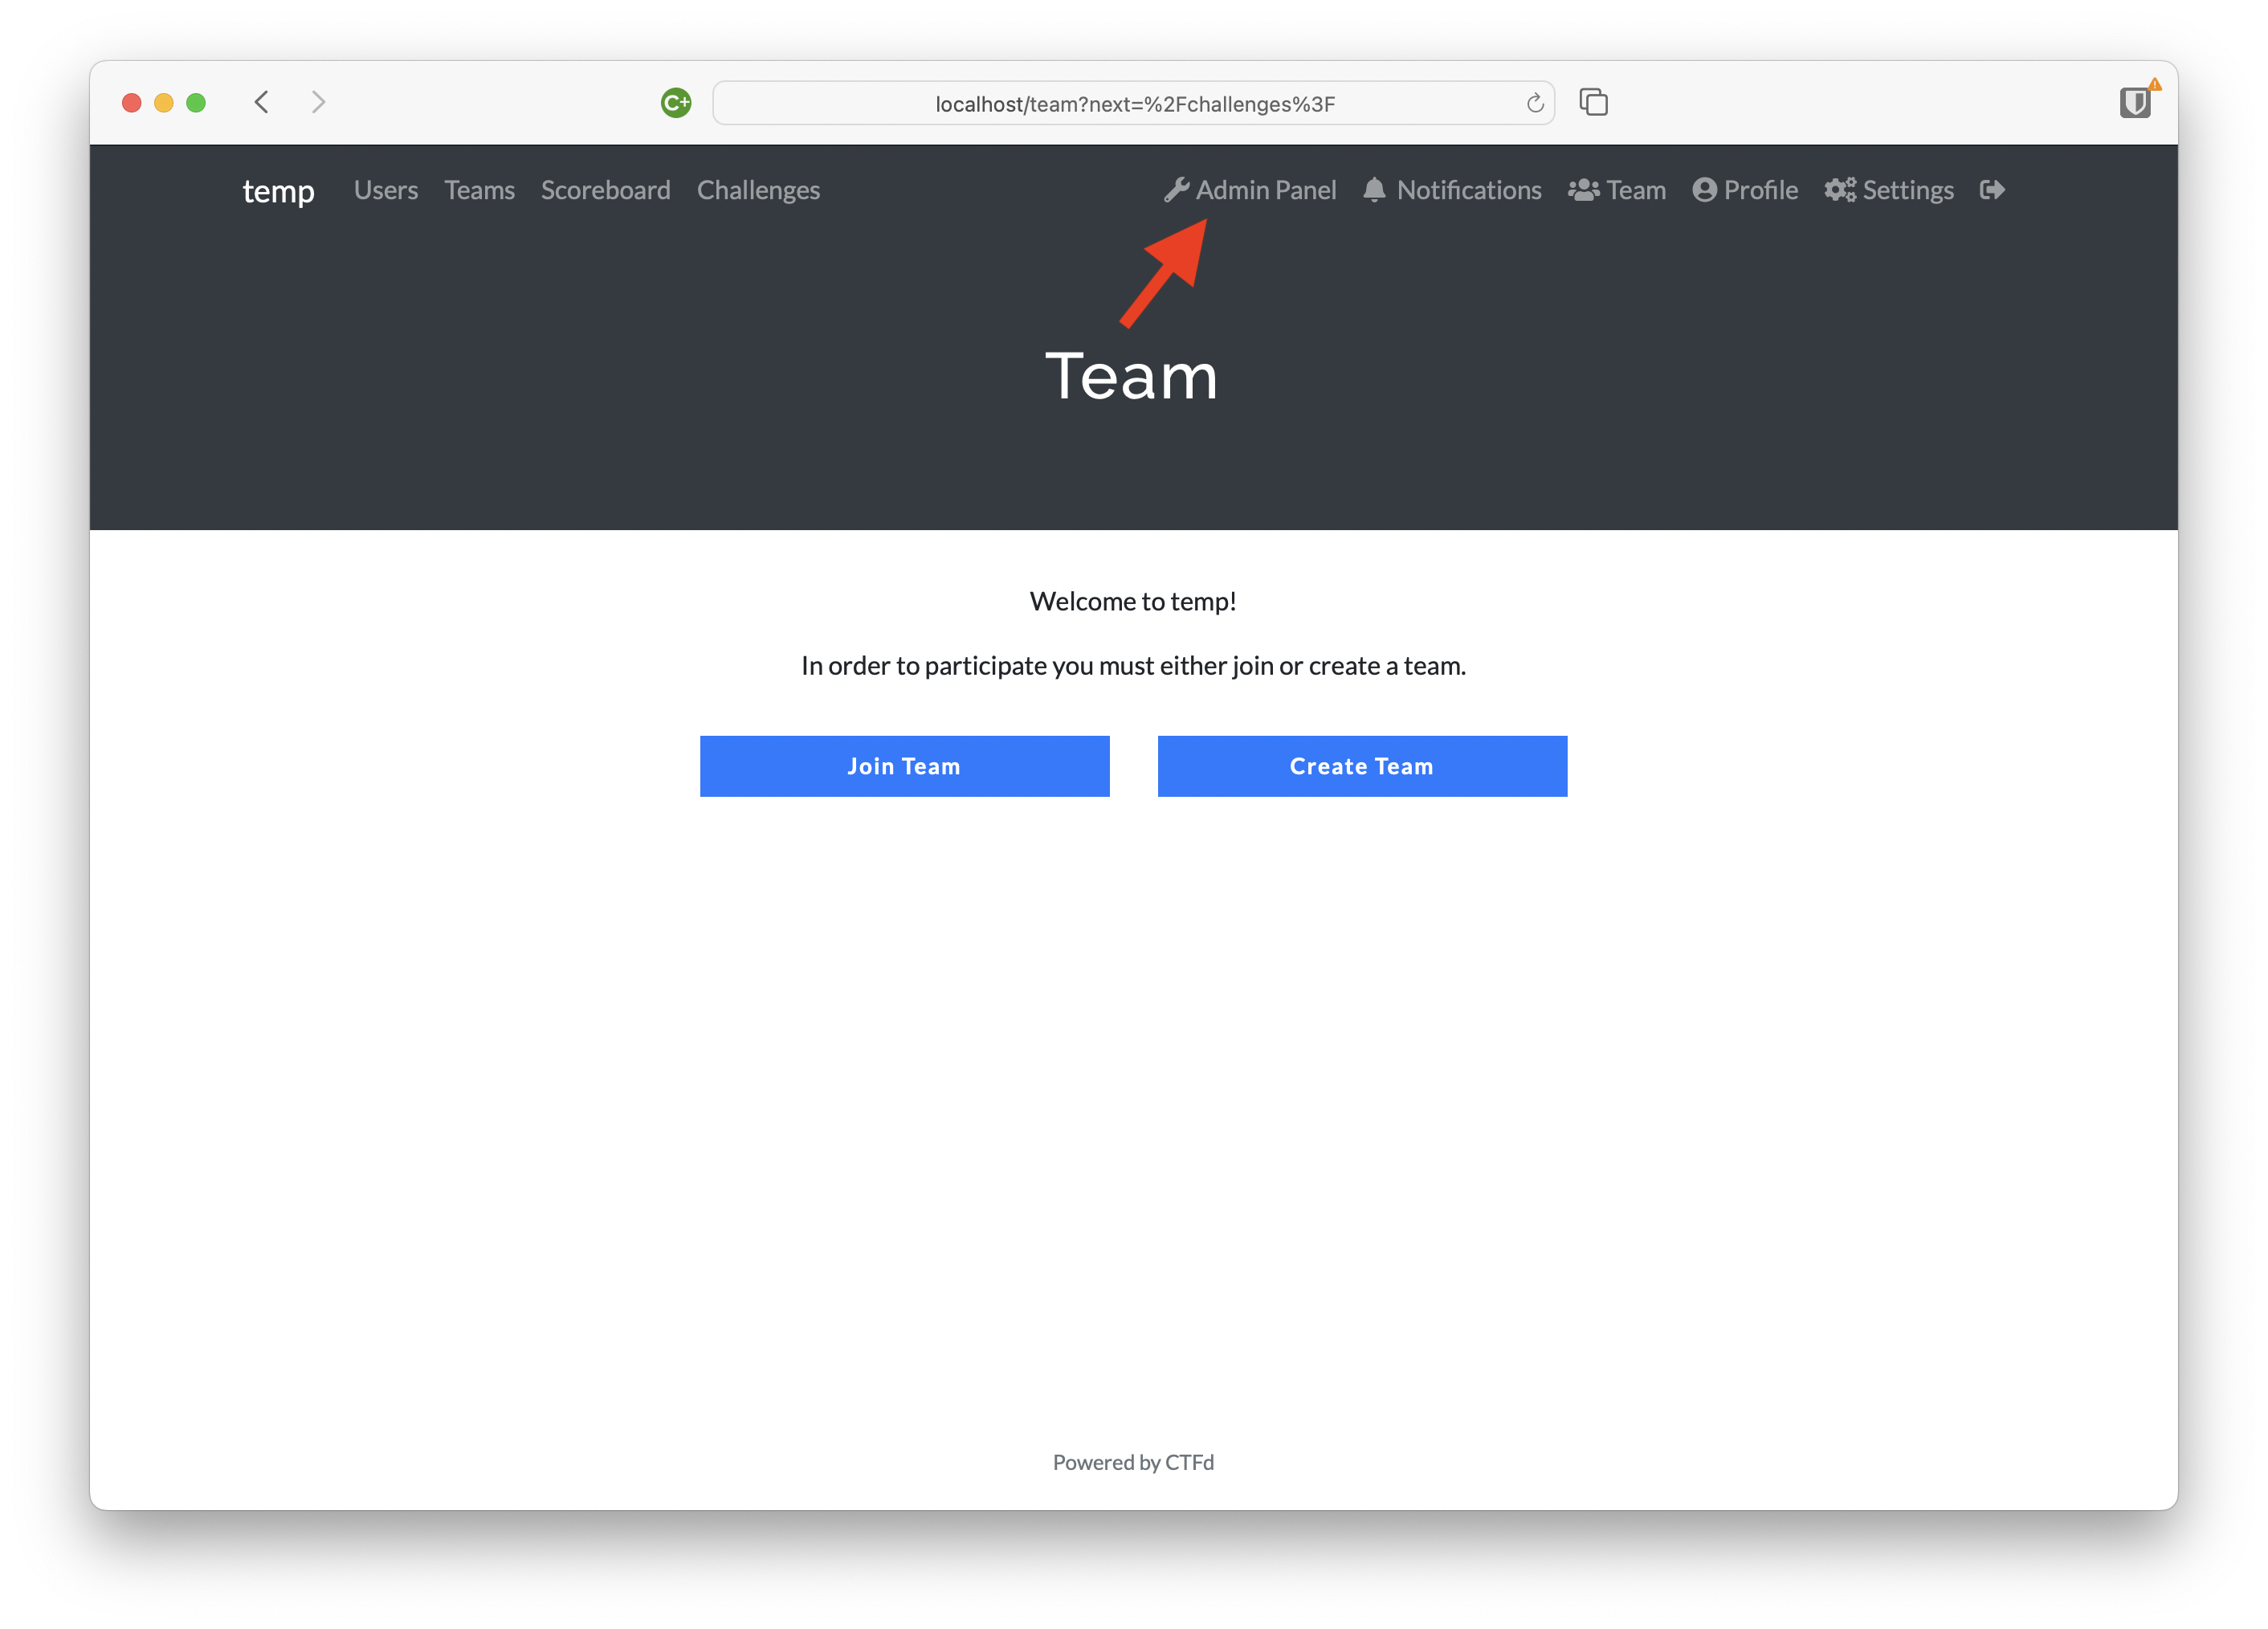
\includegraphics[width=\textwidth]{point_to_admin_panel.png}
  	   \caption{Select the Admin Panel.}
	\end{figure}
	
	\item Navigate to the ``Users'' page.
	
	\begin{figure}[H]
		\centering
	   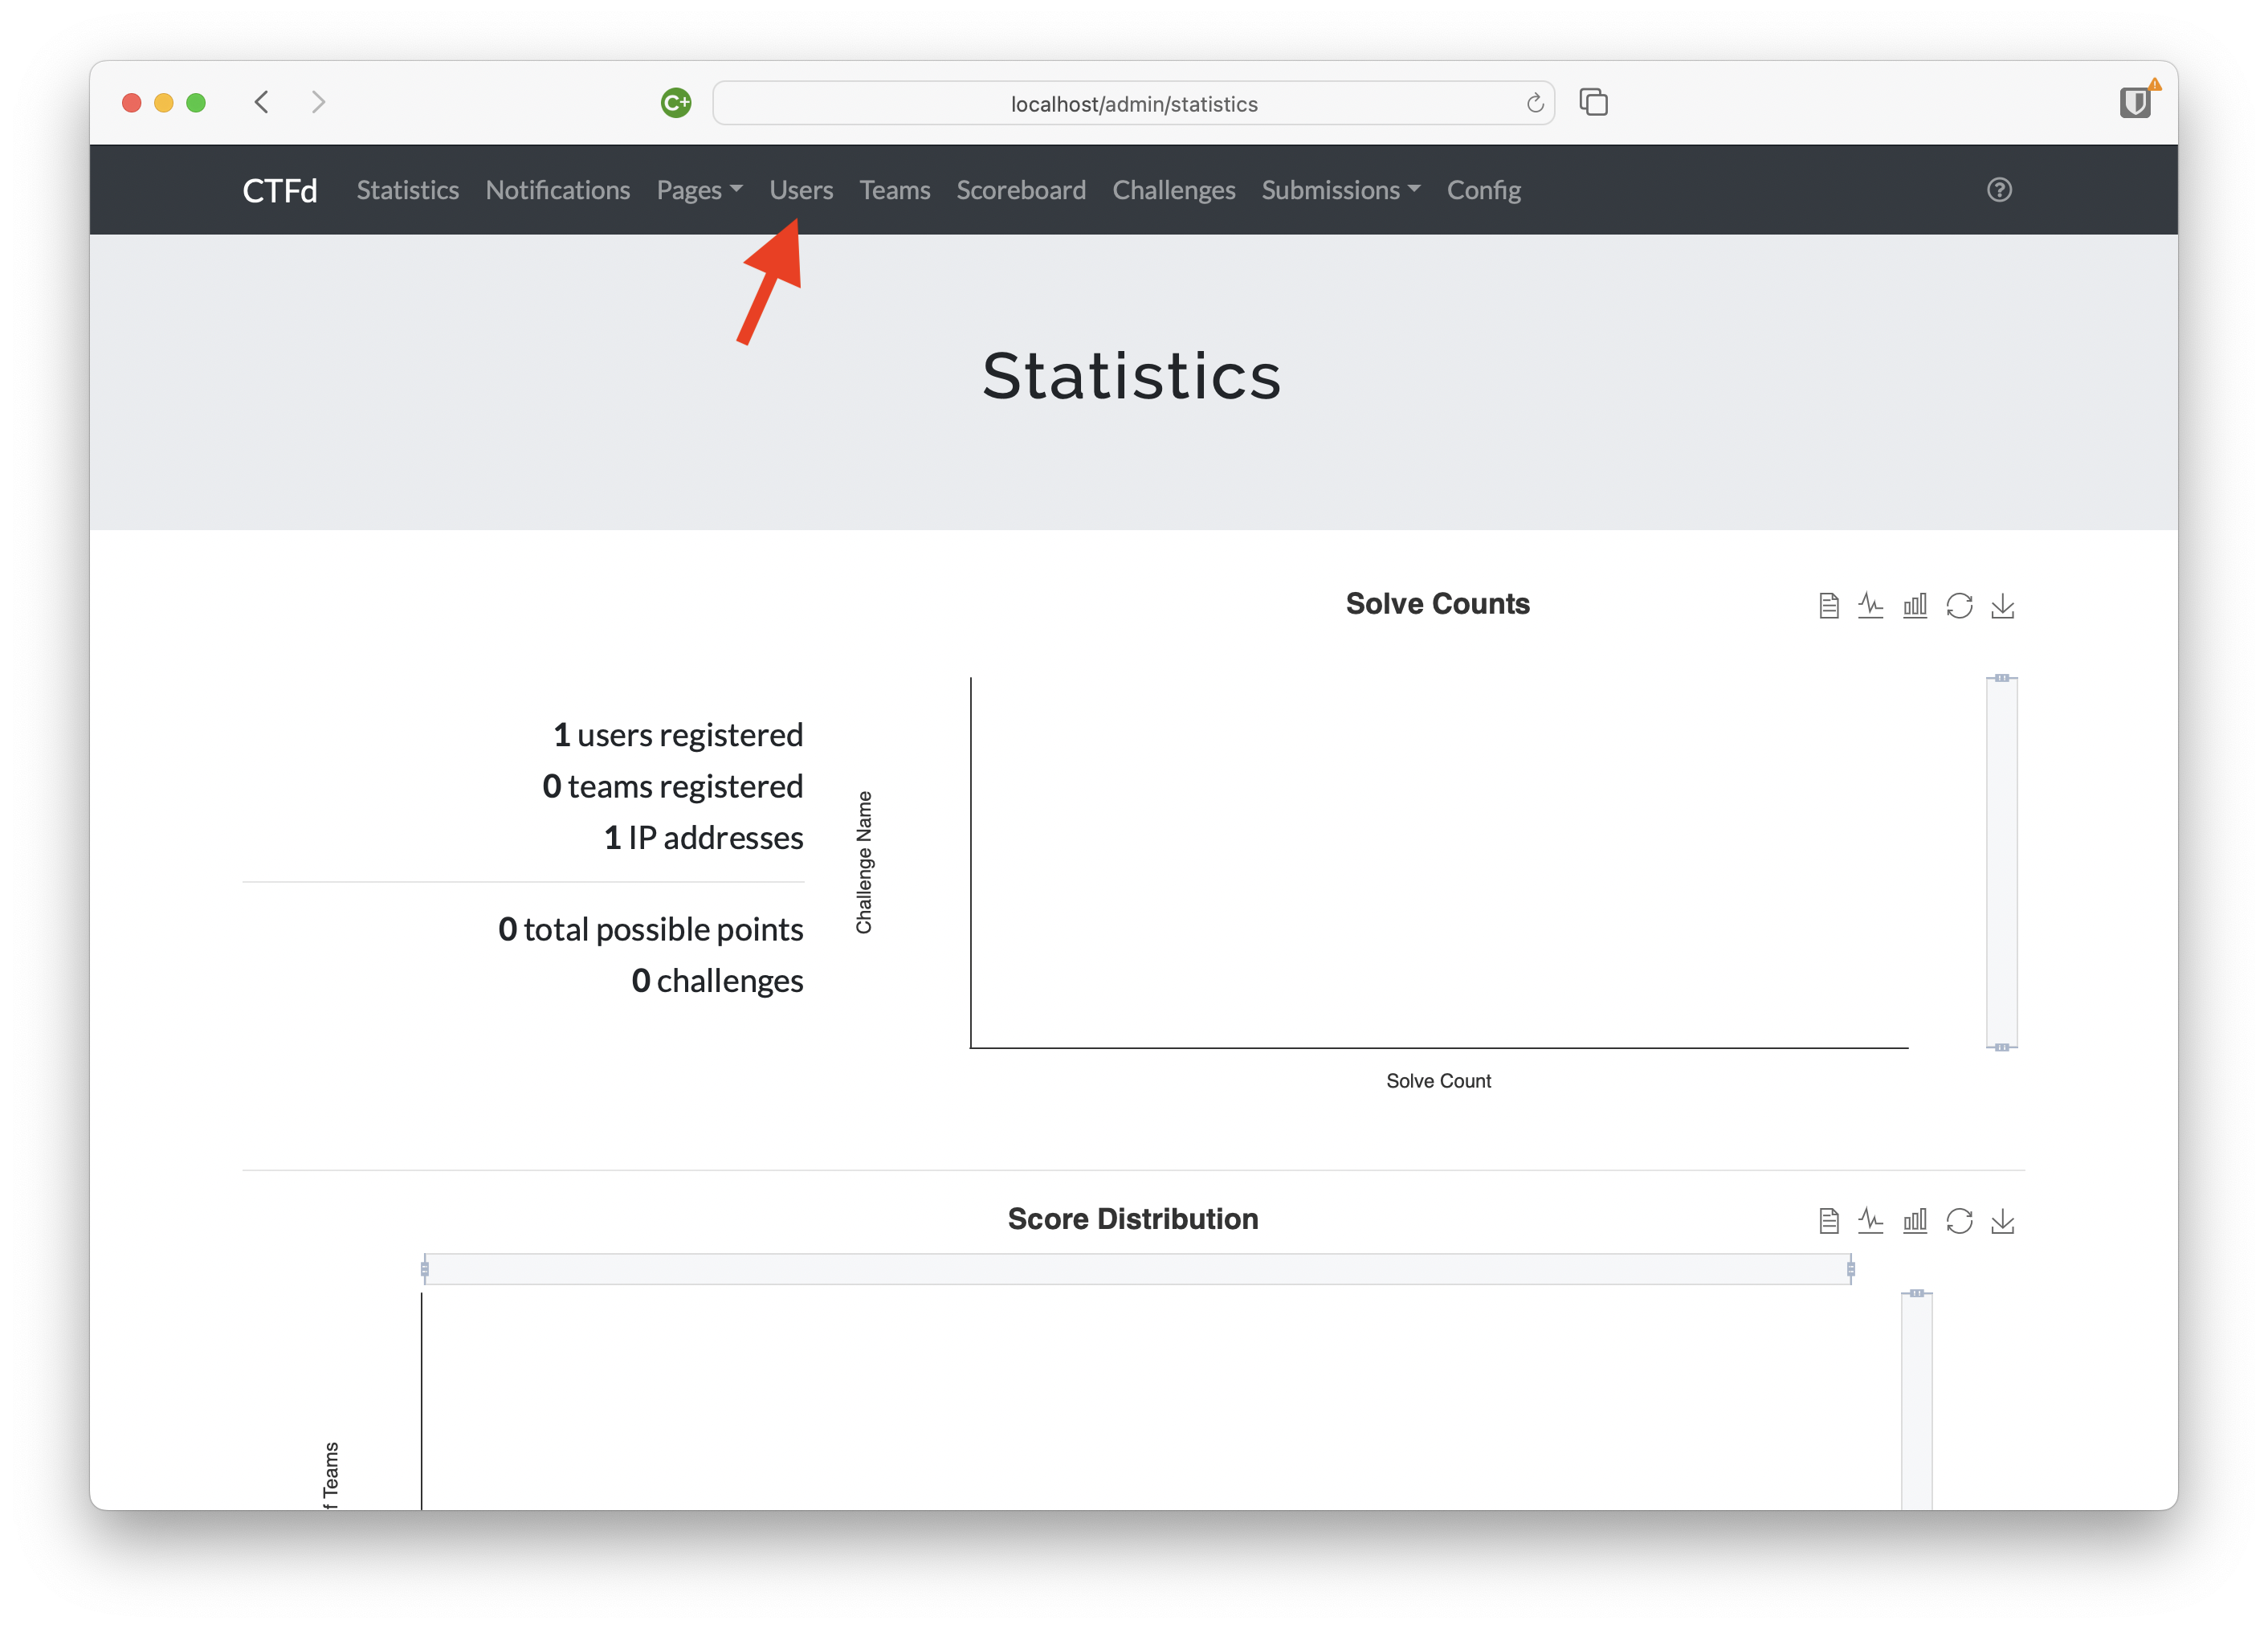
\includegraphics[width=\textwidth]{admin_panel_point_to_users.png}
  	   \caption{Select the Users page.}
	\end{figure}
	
	\item Select the $\oplus$ symbol to add a new user.
	
	\begin{figure}[H]
		\centering
	   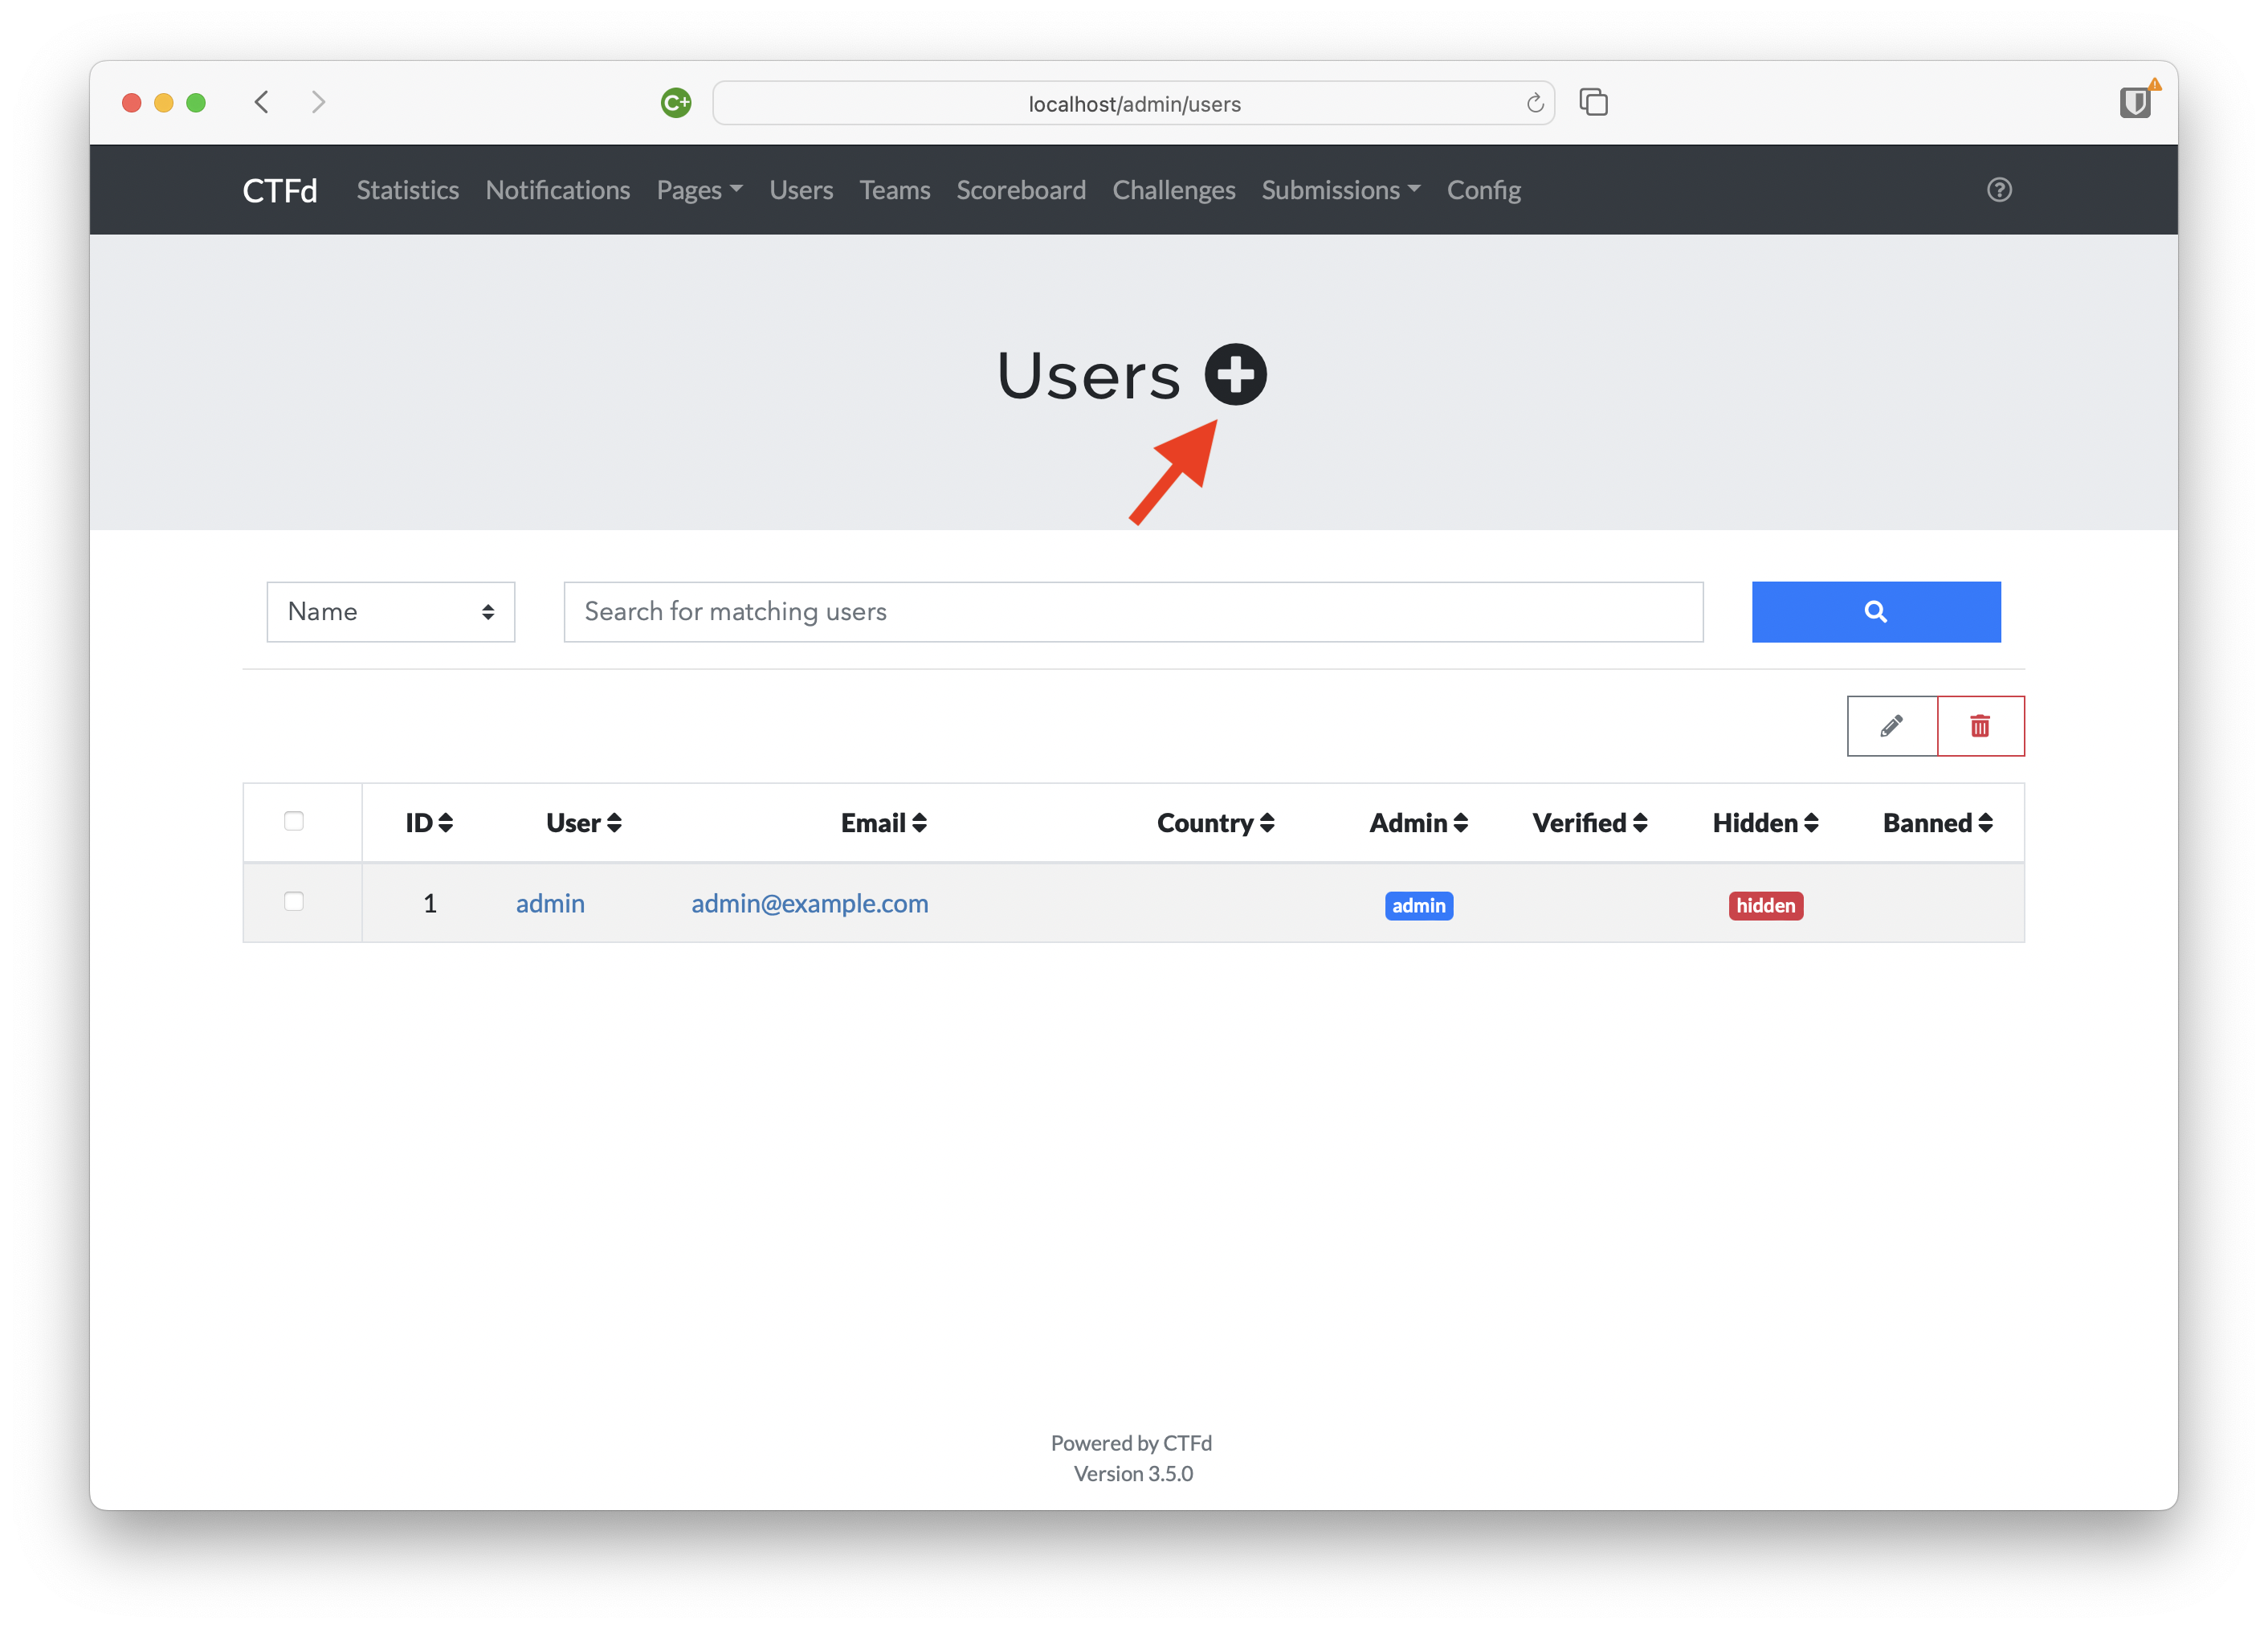
\includegraphics[width=\textwidth]{hit_plus_add_new_user.png}
  	   \caption{Select the ``plus'' symbol to add a new user.}
	\end{figure}

	\item Fill out the new user account details.
			Ensure that you set the account type to ``Admin''.
			
	\begin{figure}[H]
		\centering
	   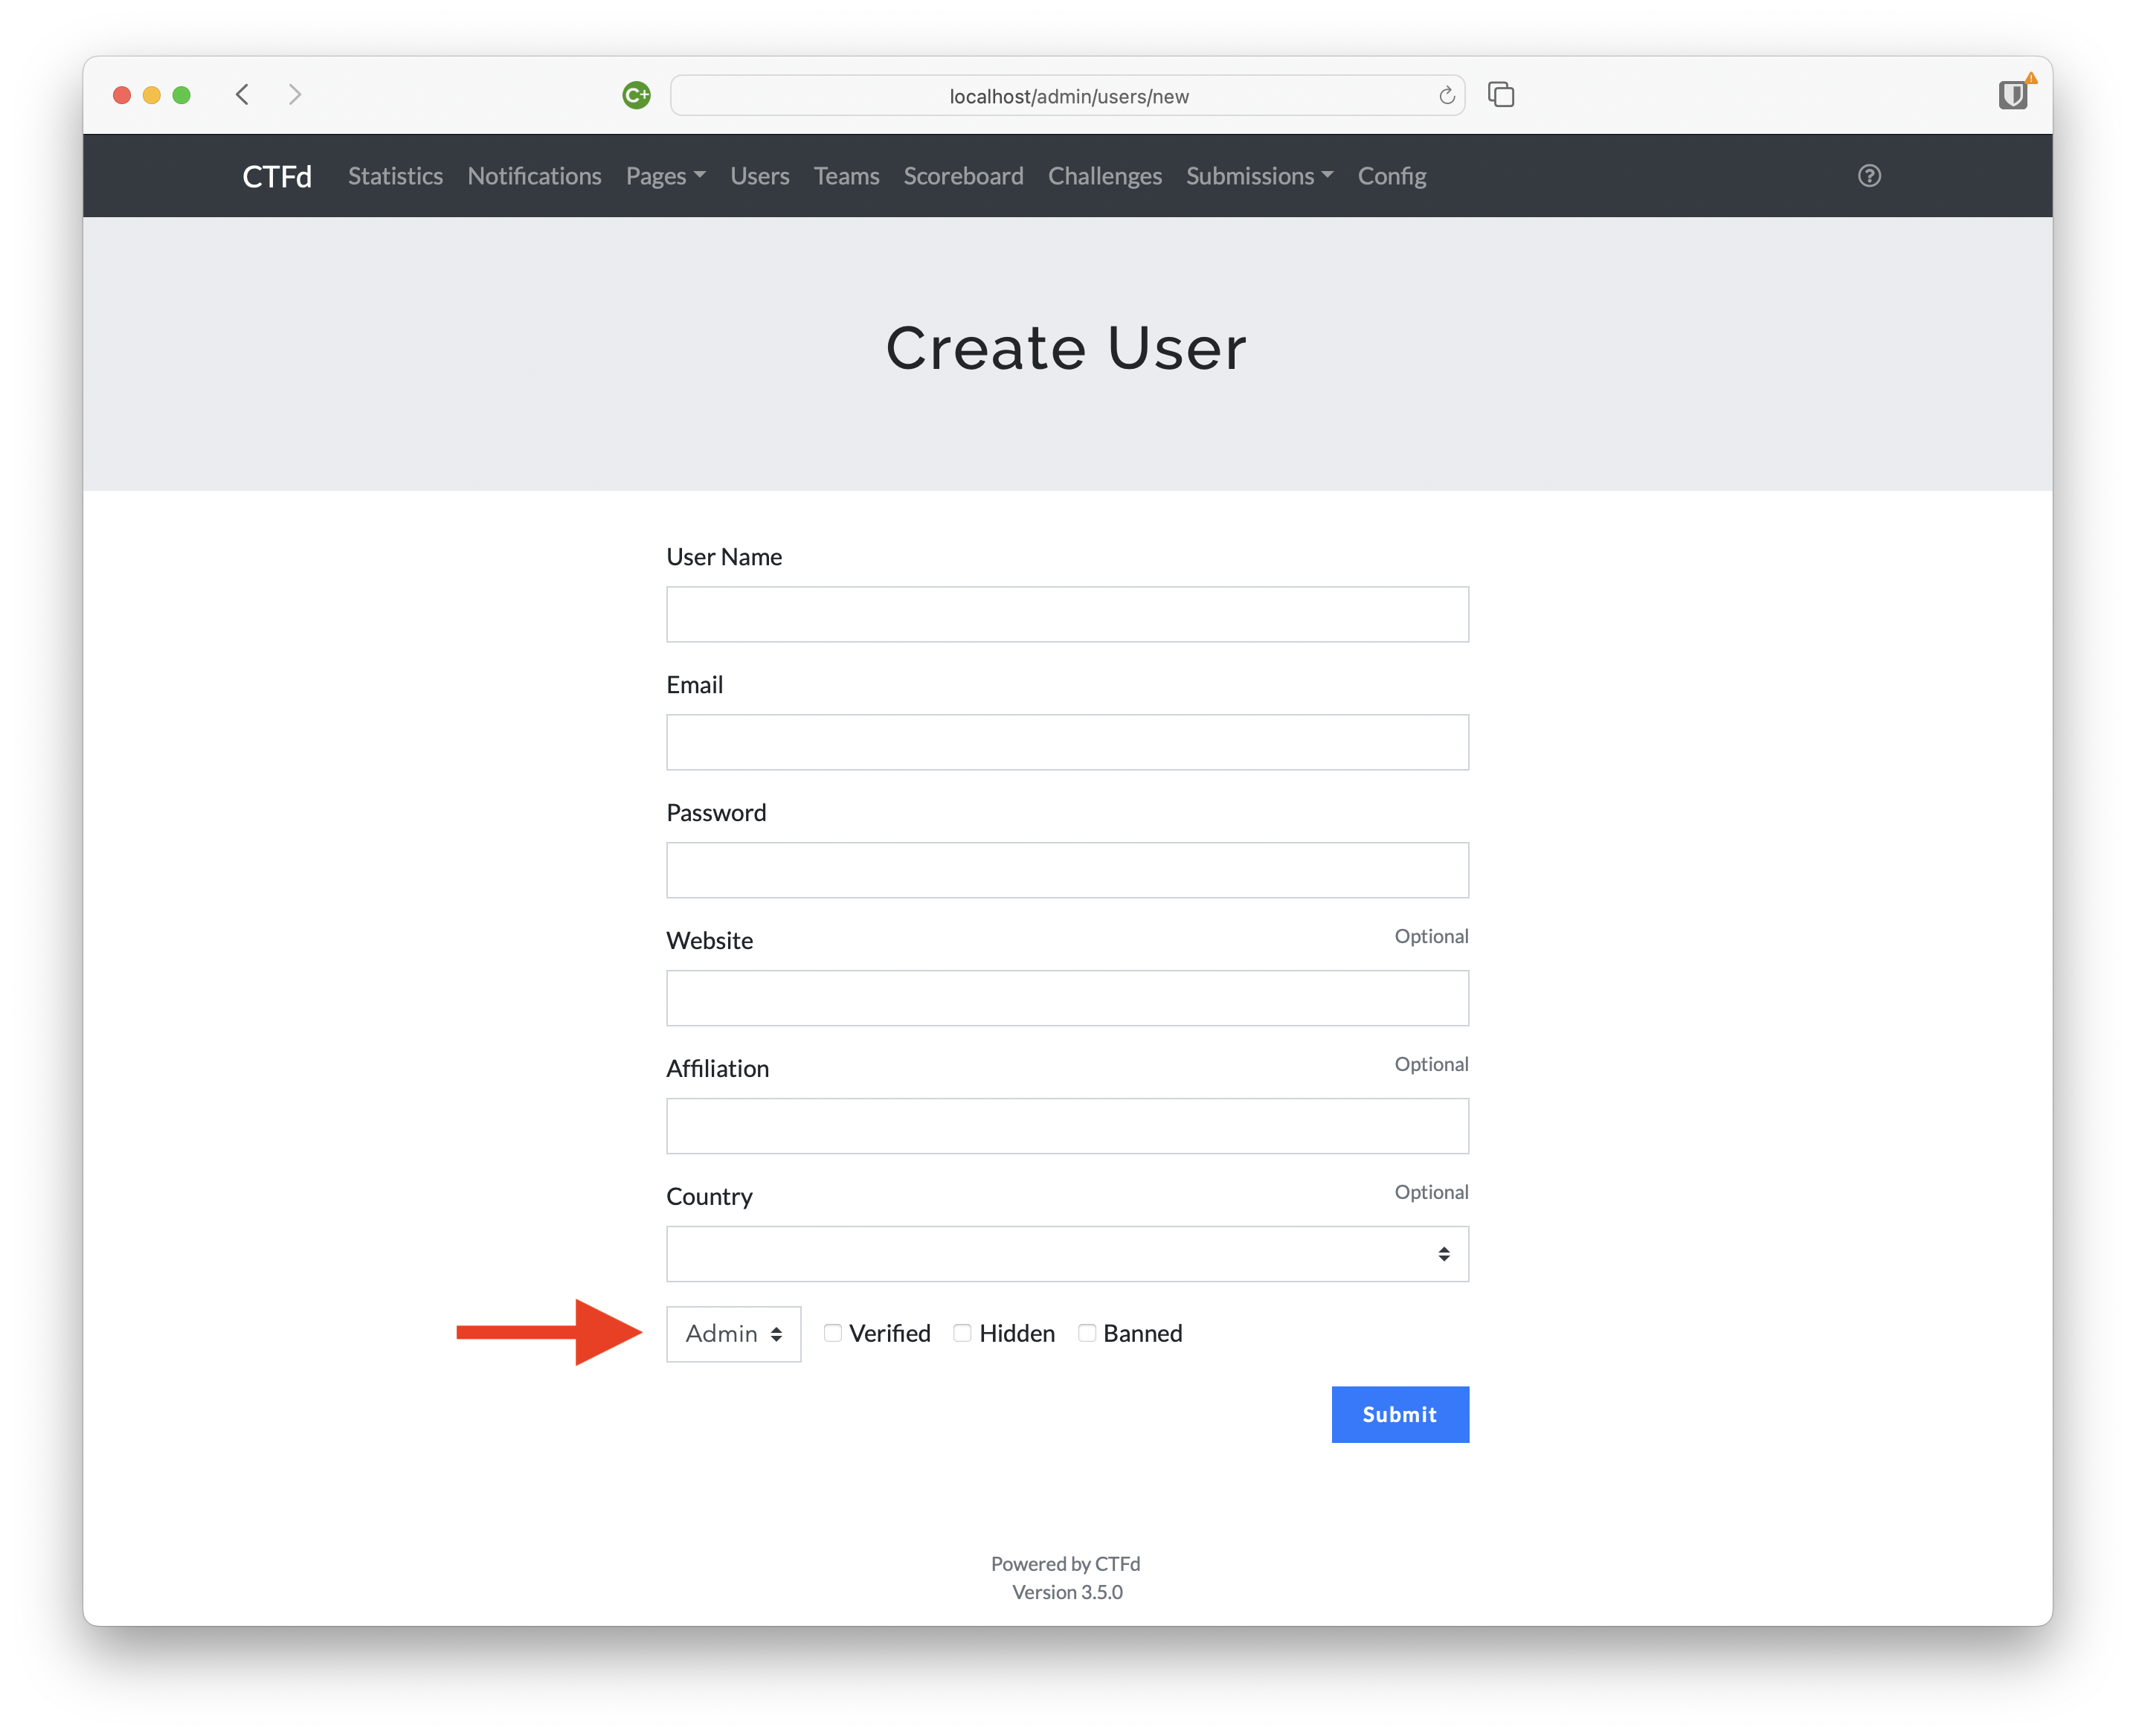
\includegraphics[width=\textwidth]{create_admin_account.png}
  	   \caption{Set the new user account type to ``Admin''.}
	\end{figure}

	\item After you have created the new Admin account, make sure to delete the old one from the ``Users'' page.
			
	\begin{figure}[H]
		\centering
	   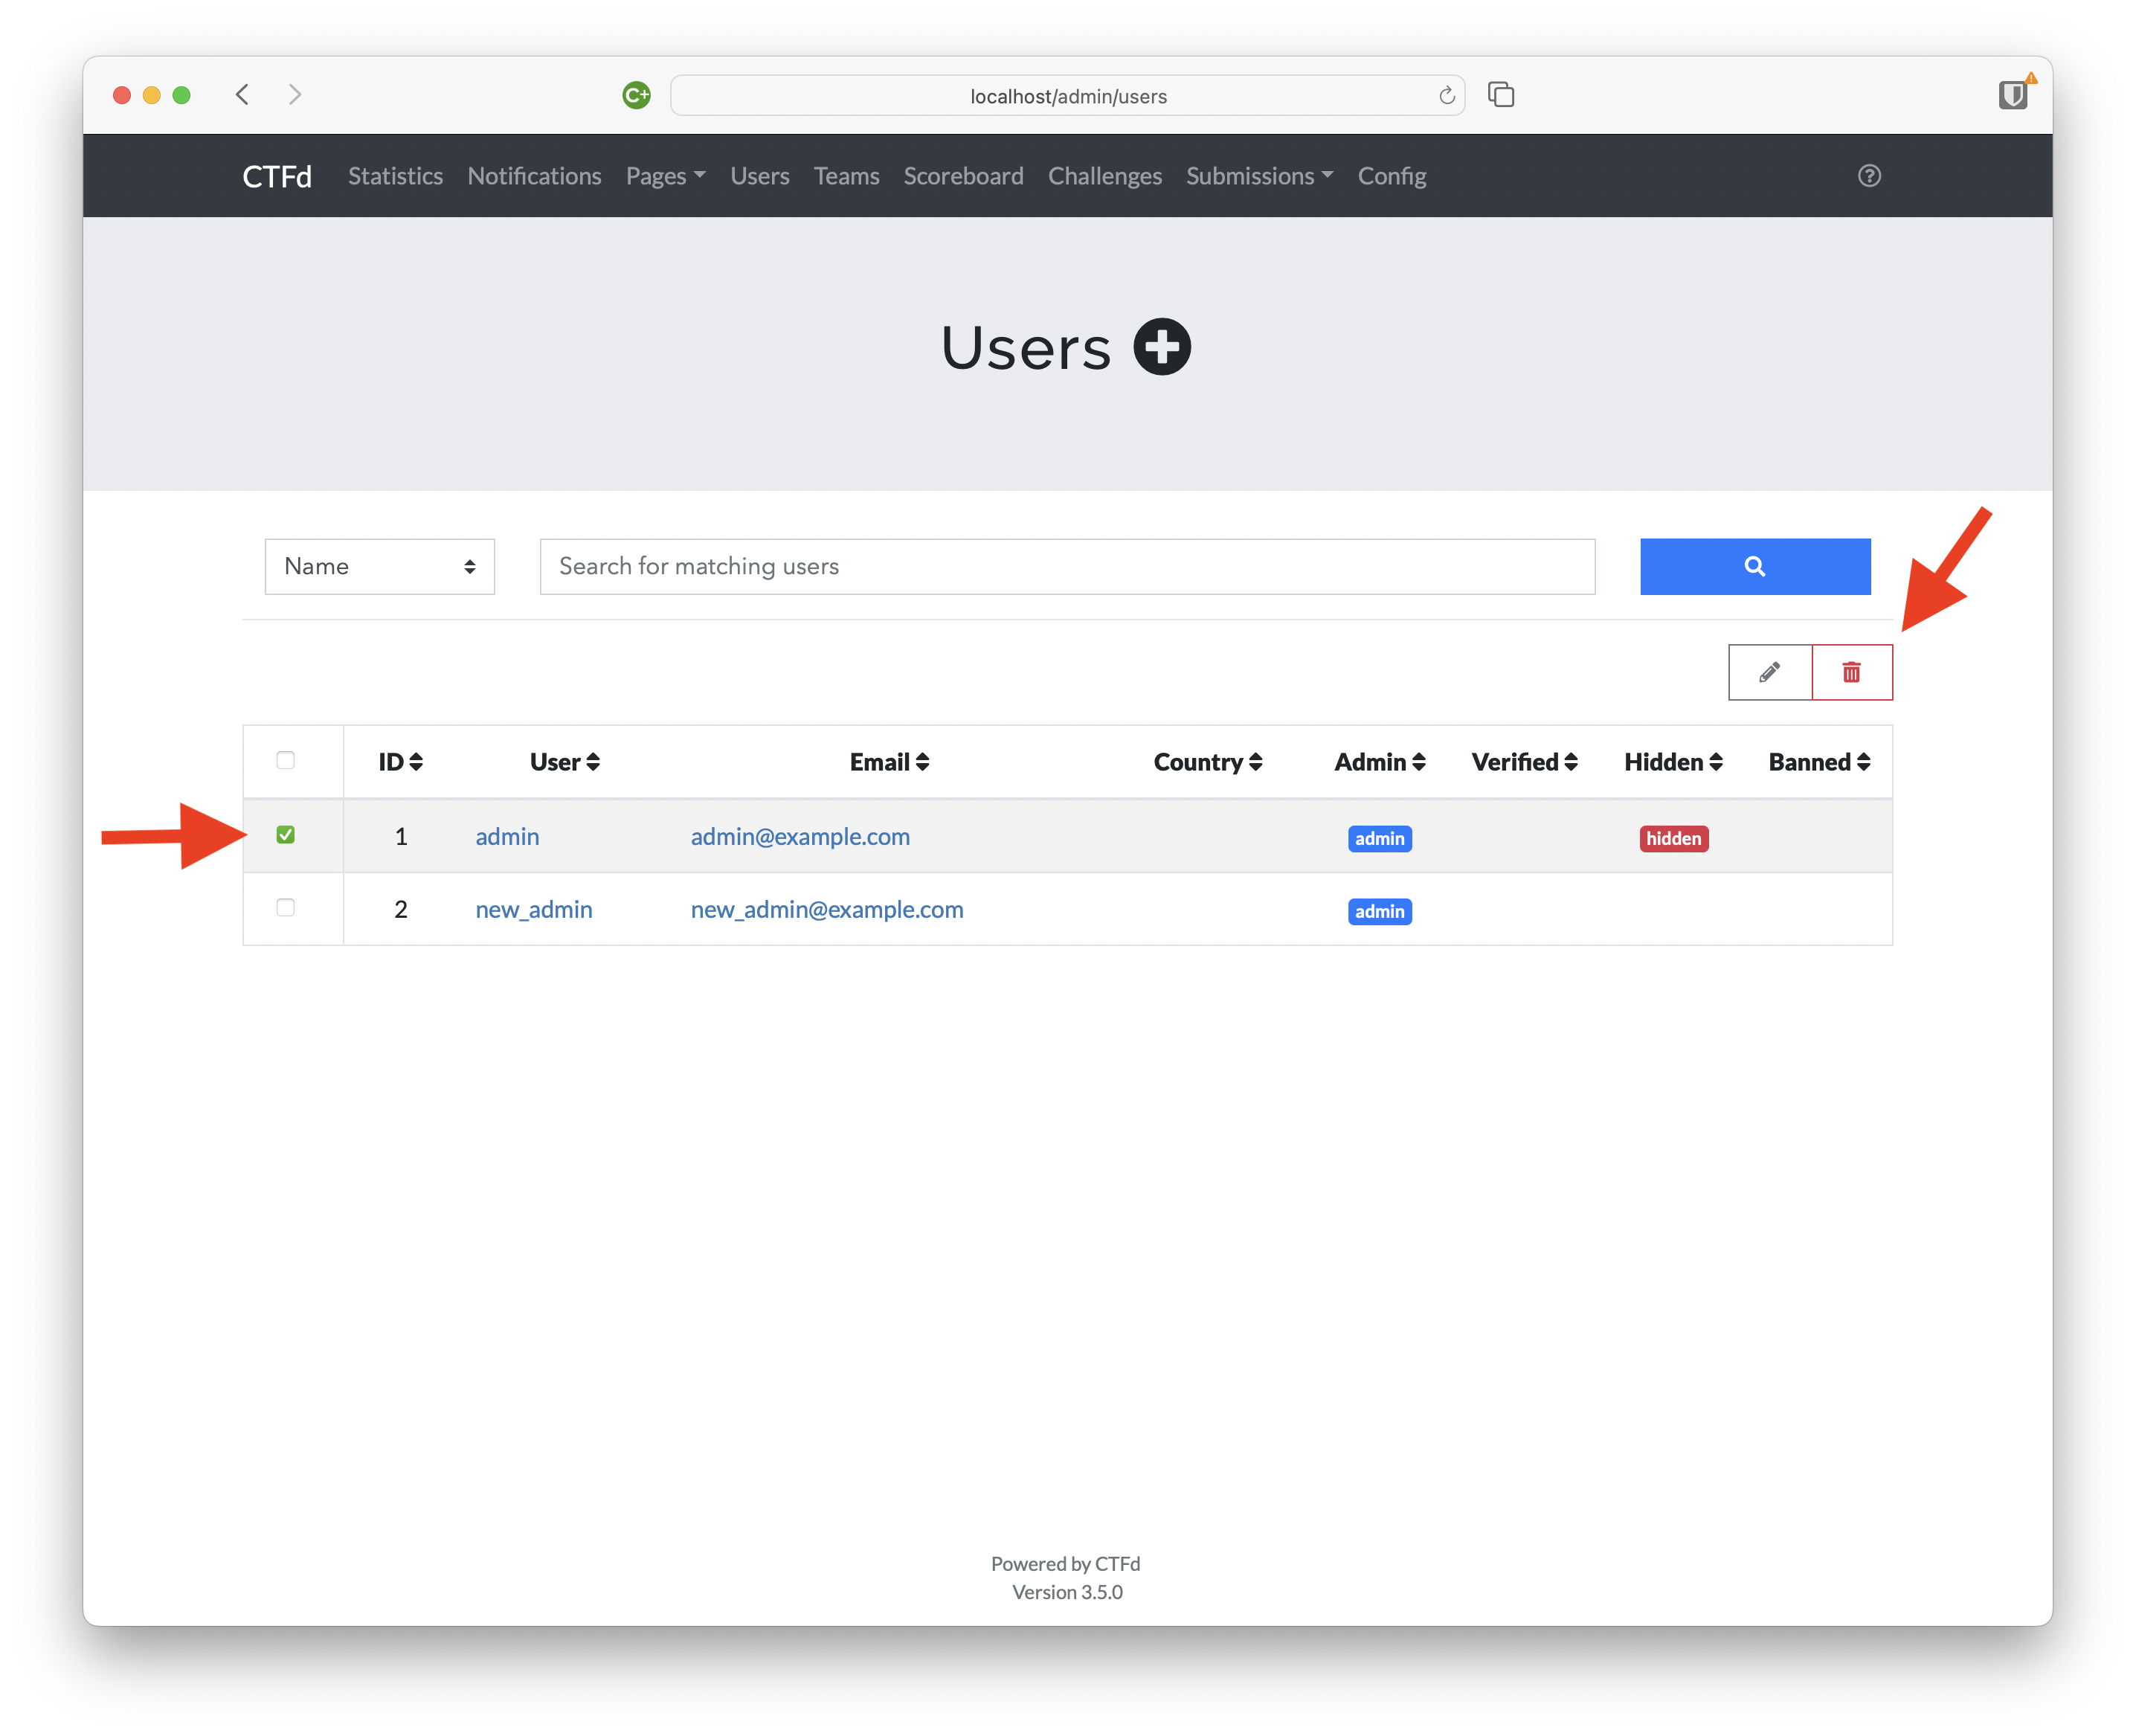
\includegraphics[width=\textwidth]{delete_old_admin.png}
  	   \caption{Delete the old Admin account.}
	\end{figure}

\end{enumerate}

\subsubsection{Importing challenges}

There are two main ways to import CTF challenges into the CTFd application.
First, make sure the CTFd application is running, then login to the admin portal using admin credentials.
Next, navigate to \texttt{Admin Panel > Config > Backup}.
From here there are two options: importing a \texttt{.zip} or importing \texttt{.csv}.
There are a few differences between the two import options:

\subsubsection{Importing challenges in \texttt{.zip} files}

\begin{itemize}
   \item \textbf{This will overwrite any existing configurations you have in place}, including user accounts, challenges, files, etc. This essentially imports a snapshot of the CTFd application at the time the \texttt{.zip} file was generated.
   \item Multiple challenges can be imported in a single \texttt{.zip} file.
   \item Files needed to complete the challenges will be included when imported.
\end{itemize}

\subsubsection{Importing challenges in \texttt{.csv} files}

\begin{itemize}
   \item This will not overwrite any existing configurations you have in place.
   \item Multiple challenges can be imported in a single \texttt{.csv} file.
   \item Files needed to complete the challenge \textbf{will not} be included when imported.
\end{itemize}

\subsubsection{Challenge Docker Containers}

Most of the CTF challenges will require spinning up a Docker container that will host the infrastructure that is unique to running that challenge.
The pertinent information for setting up challenge specific Docker containers will be included in a \texttt{README.md} file along with the other CTF challenge files.

\subsection{Management \& Troubleshooting}

Student passwords can be reset through the admin panel by clicking on the user in the ``Users'' tab.
If the server goes down, the containers for both CTFd and the docker challenges may need to be restarted. Use the same docker command from the CTFd setup instructions to launch CTFd, and use the ``start containers'' bash script in the server challenges folder to restart all challenge containers.
It is possible you may need to forcibly shut down and remove old container versions if the server restarts.
Challenges can be enabled/disabled/modified on the fly using the admin panel of the platform online.
Challenge solutions are available to instructors upon request (see bottom of page for contact info).

\section{For Students}

These instructions can be copied to students to introduce them to CTFs and inform them of how to participate in this CTF platform.
Note that you (the administrator) need to plug in the web address of the CTF server in the instructions.

\subsection{What is a CTF?}

A \href{https://en.wikipedia.org/wiki/Capture_the_flag_(cybersecurity)}{CTF (Capture The Flag)} is a kind of information security competition that can challenge contestants to solve a variety of challenges, ranging from a scavenger hunt on Wikipedia to basic programming exercises, to hacking your way into a server to steal data.
In these challenges, the contestant is usually asked to find a specific piece of text that may be hidden on the server or behind a webpage.
This goal is called the flag, \href{https://dev.to/atan/what-is-ctf-and-how-to-get-started-3f04}{hence the name}!
In the context of this class, these challenges are in CTF format, where each submission consists of a string of text.
The challenges are designed to test your mastery of the hands-on security material covered in class, as well as proficiency with the security tools used.

\subsection{How to participate}

Please navigate to the following link: [your server DNS here].
You may get a security notification that the site is not secure; if so, go to the ``advanced'' option continue anyway.
If Chrome does not work as a browser, Firefox should.
Please register a new account using your school email address and a username.
Make sure you also remember your password for future logins.
Once you log in, you should see a page with challenges for you to complete.
Use the prompts and files provided to find the flags!

\section{Credits}

\begin{itemize}
   \item Some challenges are based on existing challenges from CTF sources \href{https://www.picoctf.org/}{PicoCTF}, \href{https://www.defconbiohackingvillage.org/}{DEFCON Biohacking}, and CSICTF.
   \item This platform was originally developed by \href{mailto:zack.kaplan@wustl.edu}{Zack Kaplan} as part of a Master's project at \href{https://wustl.edu/}{Washington University in St. Louis (WUSTL)}.
   \item The work is being continued by \href{mailto:dylan.simmons@wustl.edu}{Dylan Simmons} as part of a Master's project at WUSTL.
   \item The project development is being advised by \href{mailto:svcole@wustl.edu}{Steve Cole}.
\end{itemize}

\section{Feedback and Collaboration}

We'd love to hear your feedback and work together on this project!

\begin{itemize}
   \item If you're using this platform in your class, please send us an e-mail --  we'd love to know how and where the platform is being used.
   \item If you'd like to fix a bug or generate a new challenge, you may fork this repo and initiate pull requests against it. 
   \item If you'd like to discuss the project and how you might use it in our class, please feel free to contact us directly via e-mail and we'd be happy to talk more about that.
\end{itemize}

\section{Publications}

\begin{enumerate}
   \item Zack Kaplan, Ning Zhang, and Stephen V. Cole. \href{https://doi.org/10.1145/3502717.3532153}{A Capture The Flag (CTF) Platform and Exercises for an Intro to Computer Security Class. (ACM ITiCSE'22)}
\end{enumerate}

\section{Contact Information}

Please contact \href{mailto:dylan.simmons@wustl.edu}{Dylan Simmons} or \href{mailto:svcole@wustl.edu}{Steve Cole} with any:

\begin{itemize}
   \item Requests for admin credentials for the CTF challenges
   \item Requests for CTF challenge solutions
   \item Questions
   \item Comments
   \item Suggestions
\end{itemize}

\end{document}
